\section{Our approach: DL8.5}
As identified in the introduction, DL8 has a number of weaknesses, which we will address in this section.

The most prominent of these weaknesses is that the size of the search tree considered by DL8 is unnecessarily large. Reconsider the example of Figure \ref{fig:2}, in which DL8’s pruning approach does not prune any node except from one infrequent itemset $(abc)$. We will see in this section that a new type of caching brand-and-bound search can reduce the number of itemsets considered significantly.

The pseudo-code of our new algorithm, DL8.5, is presented in Algorithm \ref{algo:2}. DL8.5 inherits a number of ideas from DL8, including the use of a cache, the recursive traversal of the space of itemsets, and the use of depth and support constraints to prune the search space.

The main distinguishing feature of DL8.5 concerns its use of bounds during the search.

In DL8.5, the recursive procedure \verb|DL8.5-Recurse| has an additional parameter, \emph{init\_ub}, which represents an upper-bound on the quality of the decision trees that the recursive procedure is expected to find. If no sufficiently good tree can be found, the procedure returns a tree of type \verb|NO TREE|. Initially, the upper-bound that is used is $+\infty$ (line 3). However, as soon as the recursive algorithm has found one decision tree, or has found a better tree than earlier known, the quality of this decision tree, calculated in line 21, is used as upper-bound for future decision trees and is communicated to the children in the search tree (line 25, line 14, 18).

The upper-bound is used to prune the search space using a test in line 17; intuitively, as soon as we have traversed one branch for an attribute, and the quality of that branch is already worse than accepted by the bound, we do not consider the second branch for that attribute.

$$Algo2
\label{algo:2}$$
\begin{algorithm}
	\DontPrintSemicolon
	\caption{$DL8.5(maxdepth, minsup)$}
	\label{algo:1}
	\textbf{struct} $BestTree\{init\_ub : float;\ tree: Tree;\ error : float\}$\;
	$cache \gets HashSet < Itemset, BestTree >$\;
	$(\tau, b) \gets \verb|DL8-Recurse|(\emptyset)$\;
	\Return $\tau$\;
	\textbf{Procedure} \texttt{DL8-Recurse}\;
	$solution \gets cache.get(I)$\;
	\If{solution was found}{
		\Return($solution.tree, solution.error$)\;
	}
	\If{$leaf\_error(I) = 0\ or\ |I| = maxdepth$}{
		\Return($make\_leaf(I), leaf\_error (I)$)\;
	}
	$(\tau, b) \gets (make\_leaf(I), leaf\_error (I))$\;
	\For{all attributes $i$}{
		\If{$|cover (I \cup \{i\})| \ge minsup$ and $|cover (I \cup \{\neg i\})| \ge minsup$}{
			$(\tau_1, e_1) \gets \texttt{DL8-Recurse}(I \cup \{i\})$\;
			\If{$e_1 \le b$}{
				$(\tau_2, e_2) \gets \texttt{DL8-Recurse}(I \cup \{i\})$\;
				\If{$e_1 + e_2 \le b$}{
					$(\tau, b) \gets (make\_tree(i, \tau_1, \tau_2), e_1 + e_2)$\;
				}
			}
		}
	}
	$cache.store(I, BestT ree(\tau, b))$\;
	\Return($\tau, b$)\;
\end{algorithm}


In line 18 we use the quality of the first branch to bound the required quality of the second branch further.

An important modification involves the interaction of the bounds with the cache. In DL8.5, we store an itemset also if no solution could be found for the given bound (line 29 is still executed even if the earlier loop did not find a tree).

In this case, the special value \verb|NO TREE| is associated with the itemset in the cache, and the upper-bound used during the last search is stored. The benefit of doing so is that at a later moment, we may reuse the fact that for a given itemset and bound, no sufficiently good decision tree can be found. In particular, in line 9, when the current bound (\emph{init\_ub}) is worse than the stored upper-bound for a \verb|NO TREE| itemset, we return the \verb|NO TREE| indicator immediately.

Other modifications in comparison with DL8 improve the anytime behavior of the algorithm. In line 6 the search can be interrupted when a time-out is reached, and line 12 offers the possibility to consider the attributes in a specific heuristic order to discover good trees more rapidly.

A number of different heuristics could be considered. In our experiments, we consider three: the original order of the attributes in the data, in increasing or in decreasing order of information gain (such as used in C4.5 and CART).

Our modifications of DL8 improve drastically the pruning of the search space. Figure \ref{fig:2} indicates which additional nodes are pruned during the execution of DL8.5 (for an alphabetic order of the attributes). At the end, 17 nodes are visited instead of 27.

\begin{figure}
	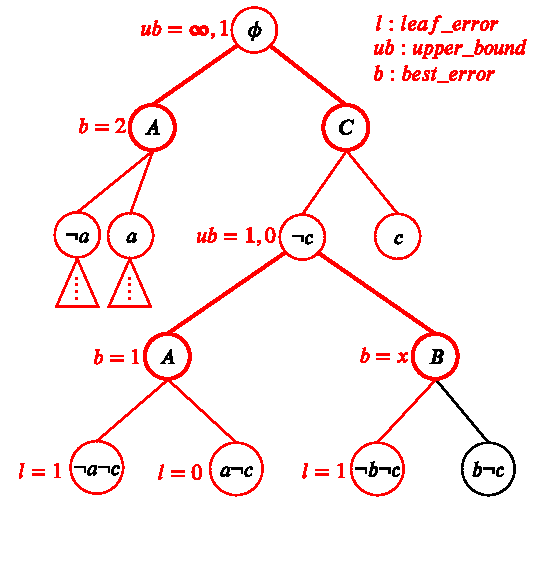
\includegraphics[width=\linewidth]{pruning}
	\caption{ Example of pruning}
\end{figure}

Figure \ref{fig:3} shows a part of the execution of DL8.5 in more detail. The initial value of the upper-bound at node $\phi$ is $+\infty$ (line 11). The attribute A provides an error of 2; the upper-bound value is subsequently updated from $+\infty$ to 1 in line 25. In the first branch for attribute C, the new value of the upper-bound is passed down recursively (line 14). Notice that the initial value of the upper-bound at node $\neg c$ is 1. At this node, the attribute A is first visited and provides an error of 1 by summing errors of $\neg a\neg c$ and $a\neg c$ (line 21). The upper-bound for subsequent attributes is then updated to 0 and passed down recursively to the first branch of attribute B. After visiting the first item $\neg b\neg c$ the obtained error is 1 and greater than the upper-bound of 0. The second item is pruned as the condition of line 18 is not satisfied. So, there is no solution by selecting the attribute B, which leads to storing the value \verb|NO TREE| for this itemset. This error value is represented in Figures 2 and 3 by the character x.

The reuse of the cache is illustrated for itemset $\neg ac$ (Figure \ref{fig:2}). The first time we encounter this itemset, we do so coming from the itemset $\neg a$ for an upper-bound of zero; after the first branch, we observe that no solution can be found for this bound, and we store \verb|NO TREE| for this itemset. The second time we encounter $\neg ac$, we do so coming from the parent c, again with an upper-bound of 0. From the cache we retrieve the fact that no solution could be found for this bound, and we skip attribute A from further consideration.